\documentclass[showtrims,		% Mostra as marcas de corte em cruz
			   trimframe,
			   openany		% Mostra as marcas de corte em linha, para conferência
			   12pt				% 8pt, 9pt, 10pt, 11pt, 12pt, 14pt, 17pt, 20pt 
			   ]{memoir}
\usepackage[brazilian,
			% english,
			% italian,
			% ngerman,
			% french,
			% russian,
			% polutonikogreek
			]{babel}
\usepackage{anyfontsize}			    % para tamanhos de fontes maiores que \Huge 
\usepackage{relsize}					% para aumentar ou diminuir fonte por pontos. Ex. \smaller[1]
\usepackage{fontspec}					% para rodar fontes do sistema
\usepackage[switch]{lineno} 			% para numerar linhas
\usepackage{lipsum}						% para colocar textos lipsum
\usepackage{alltt}						% para colocar espaços duplos. Ex: verso livre
\usepackage{graphicx}					% para colocar imagens
\usepackage{float}						% para flutuar imagens e tabelas 		
\usepackage{lettrine}					% para capsulares
\usepackage{comment}					% para comentar o código em bloco \begin{comment}...
\usepackage{adforn}						% para adornos & glyphs
\usepackage{xcolor}					 	% para texto colorido
\usepackage[babel]{microtype}			% para ajustes finos na mancha
\usepackage{enumerate,enumitem}			% para tipos diferentes de enumeração/formatação ver `edlab-extra.sty`
\usepackage{url}					% para citar sites \url
\usepackage{marginnote}					% para notas laterais
\usepackage{titlesec}					% para produzir os distanciamentos entre pontos no \dotfill

%\usepackage{makeidx} 					% para índice remissivo

\usepackage{edlab-penalties}
\usepackage{edlab-git}
\usepackage{edlab-toc}					% define sumário
\usepackage{edlab-extra}				% define epígrafe, quote
\usepackage[21x28]{edlab-margins}
\usepackage[%semcabeco, 				% para remover cabeço, sobe mancha e mantem estilos
			]{edlab-sections}			% define pagestyle (cabeço, rodapé e seções)
\usepackage[%
			% notasemlinha 			
			% notalinhalonga
			chicagofootnotes			% para notas com número e ponto cf. man. de Chicago
			]{edlab-footnotes}


\usepackage[printwatermark]{xwatermark}
\usepackage{pdfpages}
\usepackage{wrapfig}
\usepackage{tikzpagenodes}
\usepackage{textpos}
\usepackage{mdframed}
\usepackage{adjustbox}


% Medidas (ver: memoir p.11 fig.2.3)
\parindent=3ex			% Tamanho da indentação
\parskip=0pt			% Entre parágrafos
\marginparsep=-14em		% Entre mancha e nota lateral 
\marginparwidth=14em		% Tamanho da caixa de texto da nota laterial

\newcommand{\rmarginnote}[1]{\marginpar{\small\raggedleft\textcolor{rosa}{#1}}}


% Fontes
\newfontfamily\formular{Formular}
\newfontfamily\formularlight{Formular Light}
\newfontfamily\brabo{FS Brabo Pro Regular}
\setmainfont[Ligatures=TeX,Numbers=OldStyle]{Minion Pro}


% Estilos
\makeoddhead{baruch}{}{\scshape\MakeLowercase{}}{}
\makeevenhead{baruch}{}{\scshape\MakeLowercase{}}{}

\makeevenfoot{baruch}{\hspace*{-1.5cm}\small\begin{tikzpicture}[overlay]
\draw[fill=salmao,draw=none] (-11mm,-4.5mm) rectangle (4mm,4.5mm);
\node[black] at (0,0) {\thepage};
\end{tikzpicture}}{}{}

\makeoddfoot{baruch}{}{}{\hspace*{16.5cm}\small\begin{tikzpicture}[overlay]
\draw[fill=salmao,draw=none] (-4mm,-4.5mm) rectangle (11mm,4.5mm);
\node[black] at (0,0) {\thepage};
\end{tikzpicture}}

\pagestyle{baruch}		
\headstyles{baruch}

\makepagestyle{chapter}
\makeevenfoot{chapter}{\hspace*{-1.5cm}\small\begin{tikzpicture}[overlay]
\draw[fill=salmao,draw=none] (-11mm,-4.5mm) rectangle (4mm,4.5mm);
\node[black] at (0,0) {\thepage};
\end{tikzpicture}}{}{}

\makeoddfoot{chapter}{}{}{\hspace*{16.5cm}\small\begin{tikzpicture}[overlay]
\draw[fill=salmao,draw=none] (-4mm,-4.5mm) rectangle (11mm,4.5mm);
\node[black] at (0,0) {\thepage};
\end{tikzpicture}}

\usetikzlibrary{calc}

% Testes


\begin{document}


%\input{MUSSUMIPSUM}  		% Teste da classe
%!TEX root=./LIVRO.tex
% Este documento tem a ver com as partes do LIVRO. 

% Tamanhos
% \tiny
% \scriptsize
% \footnotesize
% \small 
% \normalsize
% \large 
% \Large 
% \LARGE 
% \huge
% \Huge

% Posicionamento
% \centering 
% \raggedright
% \raggedleft
% \vfill 
% \hfill 
% \vspace{Xcm}   % Colocar * caso esteja no começo de uma página. Ex: \vspace*{...}
% \hspace{Xcm}

% Estilo de página
% \thispagestyle{<<nosso>>}
% \thispagestyle{empty}
% \thispagestyle{plain}  (só número, sem cabeço)
% https://www.overleaf.com/learn/latex/Headers_and_footers

% Compilador que permite usar fonte de sistema: xelatex, lualatex
% Compilador que não permite usar fonte de sistema: latex, pdflatex

% Definindo fontes
% \setmainfont{Times New Roman}  % Todo o texto
% \newfontfamily\avenir{Avenir}  % Contexto

\begingroup\thispagestyle{empty}

\begin{textblock*}{2.625in}(0pt,0pt)%
\vspace*{-3.5cm}
%\hspace*{-4cm}\includegraphics[scale=1]{../watermarks/front9ano.pdf}
\end{textblock*}
                
              \vspace*{\fill}
              \begin{center}
              {\HUGE\textbf{Revisa SAEB}}\bigskip

              {\LARGE\textbf{7º ano: Matemática}}

              \bigskip
              \bigskip
              \bigskip

              {\Large
                            Thiago Figueiredo

                            }
              \end{center}
              \vspace*{\fill}

\endgroup
\pagebreak       % [Frontistício]
%!TEX root=./LIVRO.tex
%\newcommand{\linhalayout}[2]{{\tiny\textbf{#1}\quad#2\par}}
\newcommand{\linha}[2]{\ifdef{#2}{\linhalayout{#1}{#2}}{}}

\begingroup\tiny
\parindent=0cm
\thispagestyle{empty}

\textbf{Gerência editorial}\quad			 {Ana Mortara}\\
\textbf{Assistência editorial}\quad			 {Paula Dias}\\
\textbf{Assistência administrativa editorial}\quad {Gisele Cerchiaro}\\

\hspace{-5pt}\begin{tabular}{ll}
\textbf{Elaboração de conteúdo} & Abraão Augusto (Língua Portuguesa),	\\
								& Alessandra Domingues Juliano (Língua Portuguesa),	\\
								& Ana Paula Souza Rios (Língua Portuguesa),	\\
								& André Sanchez Astorino (Língua Portuguesa e Língua Inglesa),	\\
								& Clarissa Ayres Mendes (Língua Portuguesa),	\\
								& Eduardo Toniolo Campos (Matemática),	\\
								& Fernanda Dobashi (Língua Portuguesa),	\\
								& Guilherme Salles (Ciências Humanas),	\\
								& Letícia Leme (Ciências Humanas),	\\
								& Lucas Della Santina (Educação Física),	\\
								& Pilar Espí (Arte),	\\
								& Renata Cândido Carvalho (Ciências da Natureza),	\\
								& Thiago Figueiredo (Matemática),	\\
								& Victor Marques (Ciências da Natureza)	\\
\end{tabular}


\textbf{Edição}\quad	 {Carlos Rogério Duarte Barreiros, Fábia Alvim, Felipe Augusto Neves Silva}\\
\textbf{Preparação e revisão}\quad			 {Saíra Editorial}\\
\textbf{Coordenação de arte}\quad			 {Jorge Sallum}\\
\textbf{Editoração eletrônica}\quad			 {Paulo Henrique Pompermaier}\\
\textbf{Pesquisa iconográfica}\quad			 {Margarita Veloso}\\
\textbf{Projeto gráfico e capa}\quad		 {Luísa Marcelino} \\
\textbf{Código}\quad {\ifdef{\RevisionInfo{}}{\RevisionInfo{} (\today, \currenttime)}{001}\medskip}

\noindent\includegraphics[width=.8\textwidth]{../fichas/8POR.pdf}

\vfill

\textsc{casa de letras e gráfica ltda.}\\
Rua Fradique Coutinho, 1139, andar 2, sala 2\\
CEP 05416--011 -- São Paulo/\textsc{sp}, Brasil\\
Telefone: (11) 3914--7790\\\smallskip
www.casadeletras.com.br\\

\endgroup
\pagebreak
     % [Créditos]


%!TEX root=./LIVRO.tex
\chapter{APRESENTAÇÃO}

O \textbf{SISTEMA DE AVALIAÇÃO DA EDUCAÇÃO BÁSICA (SAEB)} É UM CONJUNTO
DE AVALIAÇÕES EXTERNAS EM LARGA ESCALA QUE PERMITE AO INSTITUTO NACIONAL
DE ESTUDOS E PESQUISAS EDUCACIONAIS ANÍSIO TEIXEIRA (INEP) REALIZAR UM
DIAGNÓSTICO DA EDUCAÇÃO BÁSICA BRASILEIRA E DE FATORES QUE PODEM
INTERFERIR NO DESEMPENHO DOS ESTUDANTES.

POR MEIO DE TESTES E QUESTIONÁRIOS, APLICADOS A CADA DOIS ANOS NA REDE
PÚBLICA E EM UMA AMOSTRA DA REDE PRIVADA, O SAEB REFLETE OS NÍVEIS DE
APRENDIZAGEM DEMONSTRADOS PELOS ESTUDANTES AVALIADOS, EXPLICANDO ESSES
RESULTADOS A PARTIR DE UMA SÉRIE DE INFORMAÇÕES CONTEXTUAIS.

O SAEB PERMITE QUE AS ESCOLAS E AS REDES MUNICIPAIS E ESTADUAIS DE
ENSINO AVALIEM A QUALIDADE DA EDUCAÇÃO OFERECIDA AOS ESTUDANTES. O
RESULTADO DA AVALIAÇÃO É UM INDICATIVO DA QUALIDADE DO ENSINO BRASILEIRO
E OFERECE SUBSÍDIOS PARA ELABORAÇÃO, MONITORAMENTO E APRIMORAMENTO DE
POLÍTICAS EDUCACIONAIS, SEMPRE COM BASE EM EVIDÊNCIAS.

AS MÉDIAS DE DESEMPENHO DOS ESTUDANTES, APURADAS NO SAEB, JUNTAMENTE COM
AS TAXAS DE APROVAÇÃO, REPROVAÇÃO E ABANDONO, APURADAS NO CENSO ESCOLAR,
COMPÕEM O ÍNDICE DE DESENVOLVIMENTO DA EDUCAÇÃO BÁSICA (IDEB).

REALIZADO DESDE 1990, O SAEB PASSOU POR UMA SÉRIE DE APRIMORAMENTOS
TEÓRICO-METODOLÓGICOS AO LONGO DAS EDIÇÕES. A EDIÇÃO DE 2019 MARCA O
INÍCIO DE UM PERÍODO DE TRANSIÇÃO ENTRE AS MATRIZES DE REFERÊNCIA
UTILIZADAS DESDE 2001 E AS NOVAS MATRIZES ELABORADAS EM CONFORMIDADE COM
A BASE NACIONAL COMUM CURRICULAR (BNCC).

\section*{REVISA SAEB: REFORÇO ESCOLAR}

COMO O PRÓPRIO NOME DIZ, A EDUCAÇÃO BÁSICA É AQUELA EM QUE SE PROMOVE A
FORMAÇÃO MAIS ESSENCIAL DOS ALUNOS. O SISTEMA DE AVALIAÇÃO DA EDUCAÇÃO
BÁSICA (SAEB) AJUDA NA DETECÇÃO DOS PONTOS FORTES E FRACOS NA FORMAÇÃO
DOS ALUNOS EM ESTADOS, EM MUNICÍPIOS, EM ESCOLAS, FUNCIONANDO COMO UM
PARÂMETRO PARA QUE PROBLEMAS SEJAM SOLUCIONADOS E PARA QUE, ANO APÓS
ANO, ESSA FORMAÇÃO EVOLUA E AJUDE NO CRESCIMENTO DESSAS ESCOLAS, DESSES
MUNICÍPIOS E DESSES ESTADOS.

A PREPARAÇÃO ADEQUADA PARA AVALIAÇÕES EM LARGA ESCALA, COMO A DO SAEB, É
IMPORTANTE PARA QUE, NO MOMENTO DA PROVA, OS ALUNOS POSSAM ESTAR ATENTOS
E TRANQUILOS PARA DAREM O MELHOR POSSÍVEL DE SEU POTENCIAL. ASSIM, UM
MATERIAL DIDÁTICO DE APOIO QUE, DE FATO, PROMOVA ESSA PREPARAÇÃO É O
MAIOR DOS ALIADOS PARA PROFESSORES E GESTORES. ESTE MATERIAL TEM
EXATAMENTE ESTA INTENÇÃO: GARANTIR UM MELHOR APROVEITAMENTO DE CADA
ESTUDANTE NA RESOLUÇÃO DE ATIVIDADES, PARA QUE CONSIGAM RESULTADOS
EXCELENTES NESSA TRAJETÓRIA DE AVALIAÇÃO.

O \textbf{REVISA SAEB} ESTÁ DIVIDIDO EM 18 VOLUMES, DISTRIBUÍDOS, AO
LONGO DO ENSINO FUNDAMENTAL, DA SEGUINTE MANEIRA:

\begin{itemize}
\item
  NOS ANOS INICIAIS, PARA O \textbf{PRIMEIRO}, O \textbf{SEGUNDO}, O
  \textbf{TERCEIRO} E O \textbf{QUARTO ANO}, E NOS ANOS FINAIS, PARA O
  \textbf{SEXTO}, O \textbf{SÉTIMO} E O \textbf{OITAVO ANO}, EXISTE UM
  VOLUME POR ANO DE LÍNGUA PORTUGUESA E EXISTE UM VOLUME POR ANO DE
  MATEMÁTICA.
\item
  O \textbf{QUINTO ANO} APRESENTA UMA ESTRUTURA ESPECIAL. EM UM VOLUME,
  APARECEM ESTES COMPONENTES: LÍNGUA PORTUGUESA, ARTE E CIÊNCIAS
  HUMANAS. EM OUTRO VOLUME, APARECEM ESTES COMPONENTES: MATEMÁTICA,
  EDUCAÇÃO FÍSICA E CIÊNCIAS DA NATUREZA.
\item
  O \textbf{NONO ANO} TAMBÉM APRESENTA UMA ESTRUTURA ESPECIAL. SÃO DOIS
  VOLUMES: UM CONTÉM LÍNGUA PORTUGUESA, ARTE, LÍNGUA INGLESA E CIÊNCIAS
  HUMANAS; O OUTRO CONTÉM MATEMÁTICA, EDUCAÇÃO FÍSICA E CIÊNCIAS DA
  NATUREZA.
\end{itemize}

CADA VOLUME, EM CADA COMPONENTE, ESTÁ DIVIDIDO EM MÓDULOS TEMÁTICOS (DE
UMA OU DUAS AULAS), E CADA MÓDULO CONTA COM A ESTRUTURA DESCRITA A
SEGUIR.

\begin{itemize}
\item
  A \textbf{ABERTURA DO MÓDULO} APRESENTA UM RESUMO TEÓRICO DE
  CONTEXTUALIZAÇÃO, VINCULADO, PRINCIPALMENTE, A HABILIDADES DAS
  MATRIZES DO SAEB, MAS TAMBÉM A ALGUMAS HABILIDADES DA BNCC QUE TÊM
  RELAÇÃO COM ESSAS PRIMEIRAS HABILIDADES.
\item
  NA SEQUÊNCIA, ABRE-SE UMA SEÇÃO DE \textbf{ATIVIDADES}, QUE CONTÉM
  EXERCÍCIOS DE MODELOS VARIADOS PARA RETOMADA E FIXAÇÃO
  DO CONTEÚDO TRAZIDO PELO MÓDULO.
\item
  NO FECHAMENTO DE CADA MÓDULO, SURGE UMA SEÇÃO CHAMADA \textbf{TREINO},
  QUE CONTÉM TRÊS ITENS (QUESTÕES NO MODELO DO INEP, QUE É O MESMO
  UTILIZADO NOS TESTES COGNITIVOS DO SAEB). CADA ITEM CHECA O
  DESENVOLVIMENTO DE UMA HABILIDADE DAS MATRIZES DO SAEB E, SEMPRE QUE
  HÁ CONEXÃO, ESTÁ VINCULADO A UMA HABILIDADE DA BNCC DO ANO
  CORRESPONDENTE.
\item
  OS VOLUMES SE ENCERRAM COM QUATRO \textbf{SIMULADOS}, PARA SEREM
  APLICADOS BIMESTRALMENTE. AO LONGO DOS QUATROS SIMULADOS, TODAS AS
  HABILIDADES DAS MATRIZES DO SAEB, EM CADA ANO, SÃO TRABALHADAS, DESDE
  QUE VINCULADAS A CONTEÚDOS PREVISTOS PELA BNCC.
\end{itemize}

\addcontentsline{toc}{chapter}{MATEMÁTICA}
%!TEX root=./LIVRO.tex
\captionsetup{font={small, it}}
\captionsetup{justification=raggedright, singlelinecheck=false}

\chapter{Apresentação}

\section{A \textit{Plataforma digital Revisa SAEB}}

% Felipe

A \textit{Plataforma digital Revisa SAEB} foi desenvolvida para alunos e
professores do 1º ao 9º ano do Ensino Fundamental. Por meio dela, os alunos
têm acesso às versões digitais do material impresso (apresentações), testes da
seção, simulados, vídeos e jogos. Já os professores, além de terem acesso ao
mesmo conteúdo que os alunos, contam com uma série de vídeos de capacitação.
Os coordenadores por sua vez, recebem relatórios de frequência e pontuação por
email ou pela plataforma.

Todo esse conteúdo da \textit{Plataforma digital} está publicado  um
sistema integrado de gestão de código aberto e abrangente, desenvolvido desde
2005. O projeto, conhecido como Odoo, oferece uma ampla gama de módulos e
recursos para a educação que podem ser personalizados e adaptados às
necessidades específicas de diferentes situações. Este mesmo sistema  é usado
em todas as escolas públicas de Portugal desde 2022, para vários fins
educacionais.\footnote{ Para saber mais sobre o uso do projeto Odoo, consulte
\href{Thinkopen Solutions
Portugal}}{https://www.odoo.com/pt_BR/partners/thinkopen-solutions-portugal-2614}

Especificamente, o sistema possui dois módulos que oferecem recursos relacionados ao \textbf{eLearning} (Cursos Online) e 
à aplicação de questionários e provas, que fazem parte da \textit{Plataforma digital Revisa SAEB}.  


\begin{figure}[t]
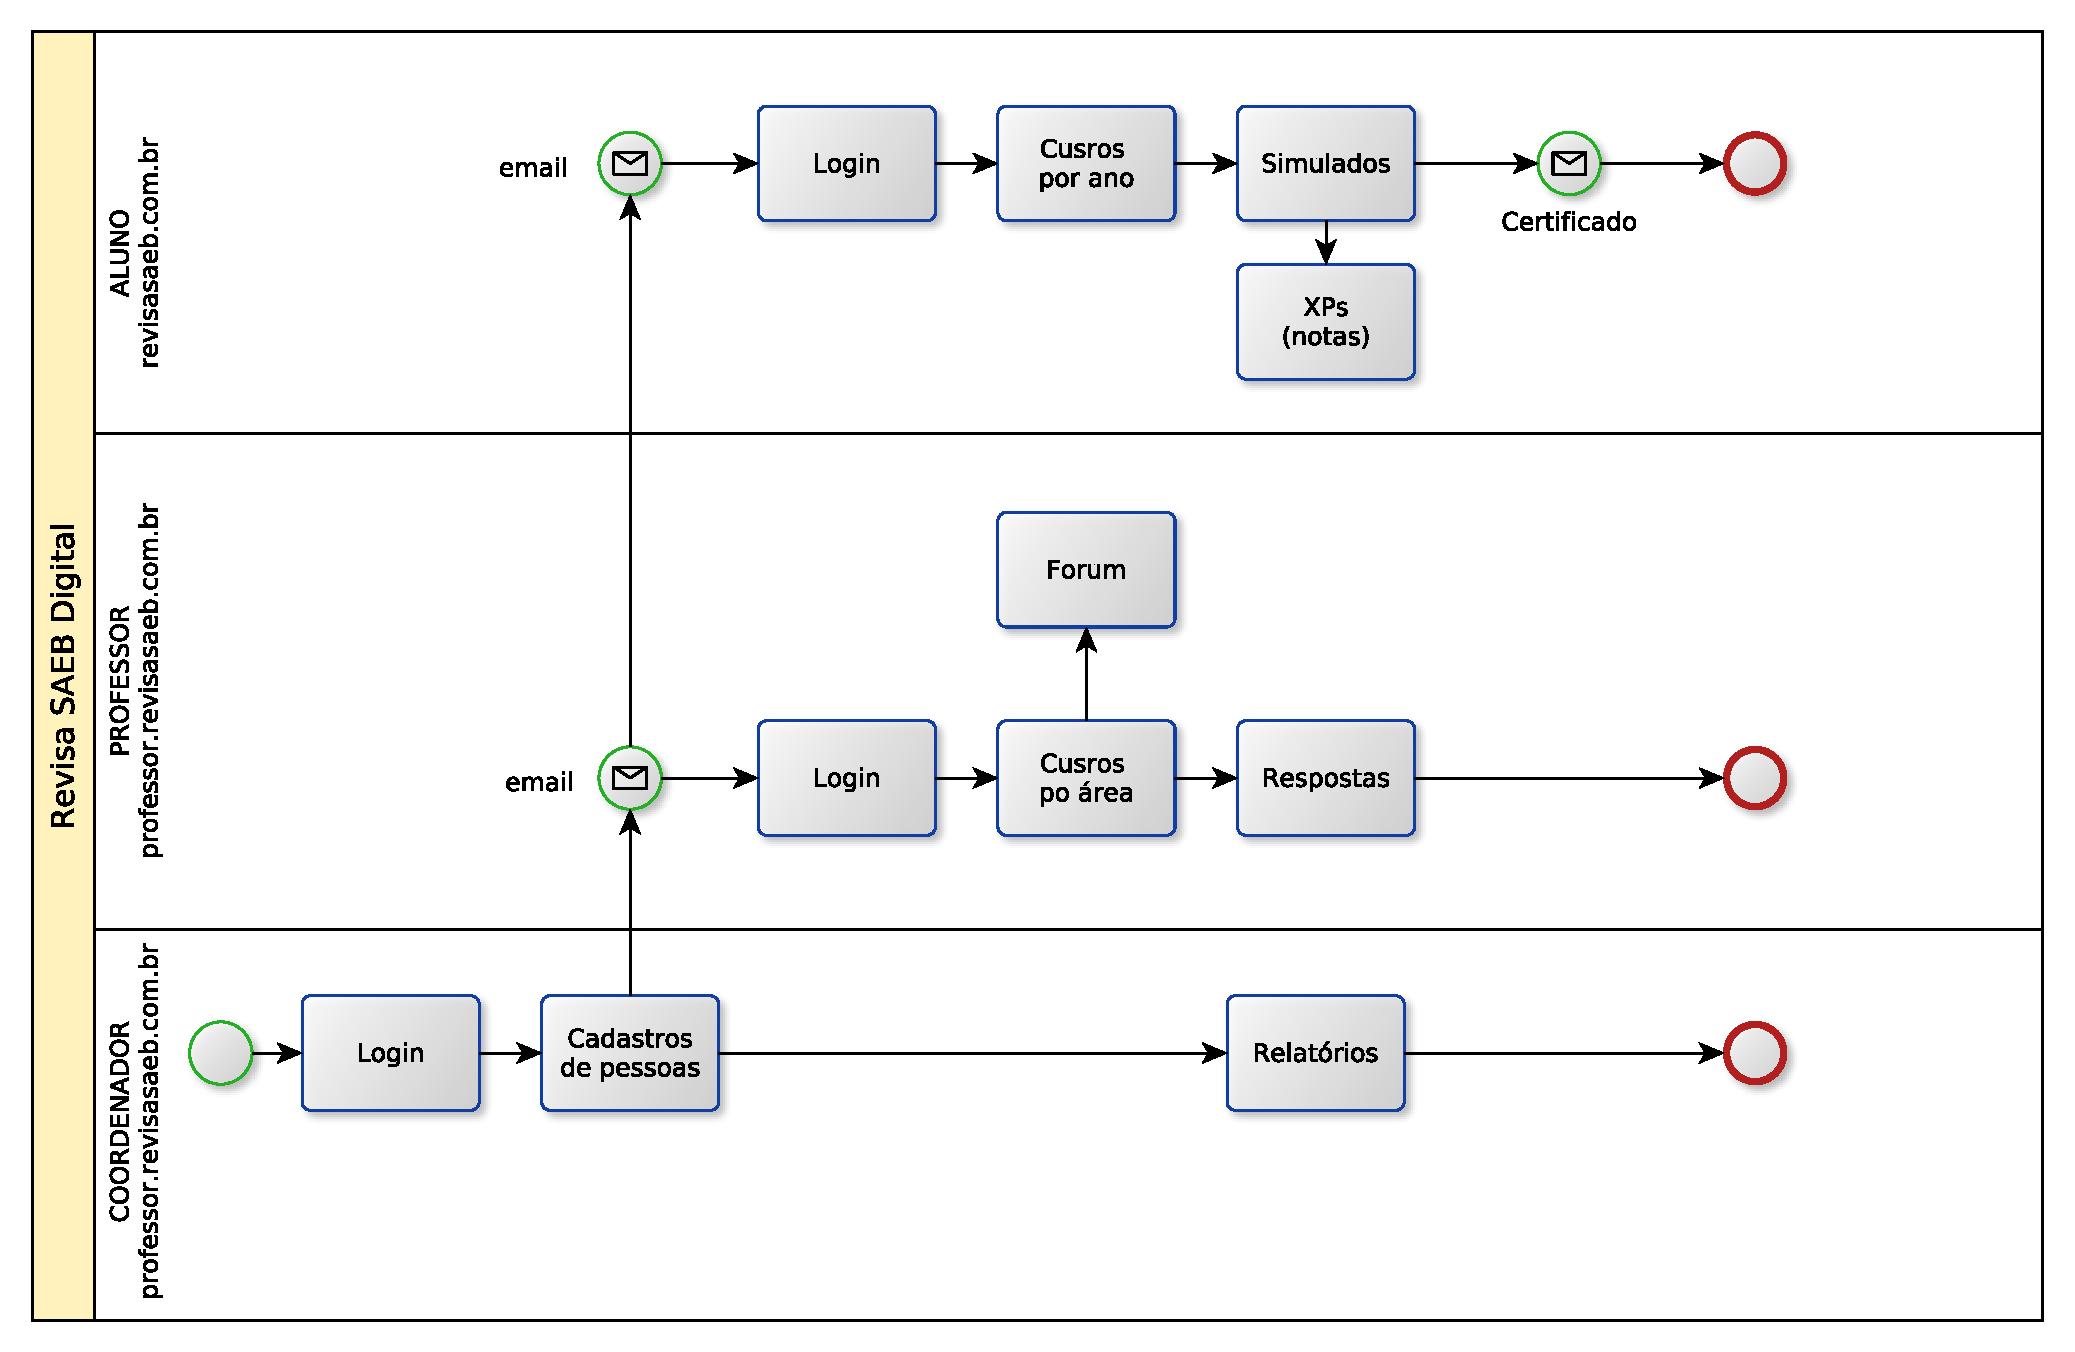
\includegraphics[width=\textwidth]{imgs/bpmn}
\caption{Estrutura da Plataforma por perfis de acesso}
\end{figure}

\section{Como acessar?} 

\begin{itemize}
\item O acesso à \textit{Plataforma Digital Revisa SAEB digital} se dá por dois endereços. \text{professor.revisasaeb.com.br} e \text{revisasaeb.com.br}.

\item E o cadastro é feito pelo coordenador ou pela importação de dados pela nossa equipe.

\item Caso o email do cadastrado seja fornecido, o sistema envia uma mensagem de boas vindas. 

\section{Quais são as áreas principais da plataforma?}

\item Após o \textit{login}, o professor terá acesso aos cursos por área e por ciclo. Ex:
Fundamental I, Matemática. Já o aluno terá acesso ao seu ano. Ex: 1º ano do Fundamental I.

\item Os cursos desdinados aos alunos incluem ainda uma seção de perguntas que servem de roteiro.
E após cada etapa concluídas, são atribuídos pontos. 

\item O relatório de frequência e desempenho fica à disposição do cooredenador e pode ser 
enviado automaticamente para o grupo de professores. 

\end{itemize}


% André
% Explicar as seções, a relação com o material impresso, os quiz






\vspace*{-3.4cm}
\hspace*{-3.7cm}\includegraphics[scale=1]{../watermarks/1simulado5ano.pdf}

%\input{Z-colofon}		   % [colofon]



\checkandfixthelayout
\end{document}
